% questions.tex —— 2004 年·全国卷Ⅲ·理科 · 题目内容片段（无答案）
% 由 tools/generate_projects.py 依来源总账自 2004/2004_数学真题_全国3理_试题.md 生成，勿手改（改源 MD 后重跑）


\begin{gktip}
\textbf{来源说明}：本题面依据固定源 PDF 两页 A3 题面逐题转录，原卷印刷页码 190–191。固定源不附答案，答案和解析均由本库独立复算。

\textbf{图形说明}：第 20 题的原卷图形关系重绘为 TikZ/PGFPlots 矢量图。
\end{gktip}

\gkpart{一、选择题（本大题共 12 小题，每小题 5 分，共 60 分．在每小题给出的四个选项中，只有一项是符合题目要求的）}

\begin{question}
\gkti{1}设集合 $M=\{(x,y)\mid x^2+y^2=1,x\in\mathbf{R},y\in\mathbf{R}\}$，$N=\{(x,y)\mid x^2-y=0,x\in\mathbf{R},y\in\mathbf{R}\}$，则集合 $M\cap N$ 中元素的个数为\mbox{（　　）}

（A）1　　（B）2　　（C）3　　（D）4

\end{question}
\begin{question}
\gkti{2}函数 $y=\left|\sin\dfrac{x}{2}\right|$ 的最小正周期是\mbox{（　　）}

（A）$\dfrac{\pi}{2}$　　（B）$\pi$　　（C）$2\pi$　　（D）$4\pi$

\end{question}
\begin{question}
\gkti{3}设数列 $\{a_n\}$ 是等差数列，且 $a_2=-6$，$a_8=6$，$S_n$ 是数列 $\{a_n\}$ 的前 $n$ 项和，则\mbox{（　　）}

（A）$S_4<S_5$　　（B）$S_4=S_5$　　（C）$S_6<S_5$　　（D）$S_6=S_5$

\end{question}
\begin{question}
\gkti{4}圆 $x^2+y^2-4x=0$ 在点 $P(1,\sqrt{3})$ 处的切线方程为\mbox{（　　）}

（A）$x+\sqrt{3}y-2=0$　　（B）$x+\sqrt{3}y-4=0$

（C）$x-\sqrt{3}y+4=0$　　（D）$x-\sqrt{3}y+2=0$

\end{question}
\begin{question}
\gkti{5}函数 $y=\sqrt{\log_{\frac{1}{2}}(x^2-1)}$ 的定义域为\mbox{（　　）}

（A）$[-\sqrt{2},-1)\cup(1,\sqrt{2}]$　　（B）$(-\sqrt{2},-1)\cup(1,\sqrt{2})$

（C）$[-2,-1)\cup(1,2]$　　（D）$(-2,-1)\cup(1,2)$

\end{question}
\begin{question}
\gkti{6}设复数 $z$ 的辐角主值为 $\dfrac{2\pi}{3}$，虚部为 $\sqrt{3}$，则 $z^2=$\mbox{（　　）}

（A）$-2-2\sqrt{3}\mathrm{i}$　　（B）$-2\sqrt{3}-2\mathrm{i}$

（C）$2+2\sqrt{3}\mathrm{i}$　　（D）$2\sqrt{3}+2\mathrm{i}$

\end{question}
\begin{question}
\gkti{7}设双曲线的焦点在 $x$ 轴上，两条渐近线为 $y=\pm\dfrac{1}{2}x$，则该双曲线的离心率 $e=$\mbox{（　　）}

（A）5　　（B）$\sqrt{5}$　　（C）$\dfrac{\sqrt{5}}{2}$　　（D）$\dfrac{\sqrt{5}}{4}$

\end{question}
\begin{question}
\gkti{8}不等式 $1<|x+1|<3$ 的解集为\mbox{（　　）}

（A）$(0,2)$　　（B）$(-2,0)\cup(2,4)$

（C）$(-4,0)$　　（D）$(-4,-2)\cup(0,2)$

\end{question}
\begin{question}
\gkti{9}正三棱锥的底面边长为 2，侧面均为直角三角形，则此三棱锥的体积为\mbox{（　　）}

（A）$\dfrac{2\sqrt{2}}{3}$　　（B）$\sqrt{2}$　　（C）$\dfrac{\sqrt{2}}{3}$　　（D）$\dfrac{4\sqrt{2}}{3}$

\end{question}
\begin{question}
\gkti{10}在 $\triangle ABC$ 中，$AB=3$，$BC=\sqrt{13}$，$AC=4$，则边 $AC$ 上的高为\mbox{（　　）}

（A）$\dfrac{3\sqrt{2}}{2}$　　（B）$\dfrac{3\sqrt{3}}{2}$　　（C）$\dfrac{3}{2}$　　（D）$3\sqrt{3}$

\end{question}
\begin{question}
\gkti{11}设函数 $f(x)=\begin{cases}(x+1)^2,&x<1,\\ 4-\sqrt{x-1},&x\geqslant 1,\end{cases}$ 则使得 $f(x)\geqslant 1$ 的自变量 $x$ 的取值范围为\mbox{（　　）}

（A）$(-\infty,-2]\cup[0,10]$　　（B）$(-\infty,-2]\cup[0,1]$

（C）$(-\infty,-2]\cup[1,10]$　　（D）$[-2,0]\cup[1,10]$

\end{question}
\begin{question}
\gkti{12}将 4 名教师分配到 3 所中学任教，每所中学至少 1 名，则不同的分配方案共有\mbox{（　　）}

（A）12 种　　（B）24 种　　（C）36 种　　（D）48 种

\end{question}
\gkpart{二、填空题（本大题共 4 小题，每小题 4 分，共 16 分．把答案填在横线上）}

\begin{question}
\gkti{13}用平面 $\alpha$ 截半径为 $R$ 的球，如果球心到平面 $\alpha$ 的距离为 $\dfrac{R}{2}$，那么截得小圆的面积与球的表面积的比值为 $\underline{\hspace{3cm}}$。

\end{question}
\begin{question}
\gkti{14}函数 $y=\sin x+\sqrt{3}\cos x$ 在区间 $\left[0,\dfrac{\pi}{2}\right]$ 上的最小值为 $\underline{\hspace{3cm}}$。

\end{question}
\begin{question}
\gkti{15}已知函数 $y=f(x)$ 是奇函数，当 $x\geqslant 0$ 时，$f(x)=3^x-1$，设 $f(x)$ 的反函数是 $y=g(x)$，则 $g(-8)=$ $\underline{\hspace{3cm}}$。

\end{question}
\begin{question}
\gkti{16}设 $P$ 是曲线 $y^2=4(x-1)$ 上的一个动点，则点 $P$ 到点 $(0,1)$ 的距离与点 $P$ 到 $y$ 轴的距离之和的最小值为 $\underline{\hspace{3cm}}$。

\end{question}
\gkpart{三、解答题（本大题共 6 小题，共 74 分．解答应写出文字说明、证明过程或演算步骤）}

\begin{question}
\gkti{17}（本小题满分 12 分）

已知 $\alpha$ 为锐角，且 $\tan\alpha=\dfrac{1}{2}$，求 $\dfrac{\sin 2\alpha\cos\alpha-\sin\alpha}{\sin 2\alpha\cos 2\alpha}$ 的值。

\end{question}
\begin{question}
\gkti{18}（本小题满分 12 分）

解方程：$4^x+|1-2^x|=11$。

\end{question}
\begin{question}
\gkti{19}（本小题满分 12 分）

某村计划建造一个室内面积为 $800\text{ m}^2$ 的矩形蔬菜温室。在温室内，沿左、右两侧与后侧内墙各保留 $1\text{ m}$ 宽的通道，沿前侧内墙保留 $3\text{ m}$ 宽的空地。当矩形温室的边长各为多少时，蔬菜的种植面积最大？最大种植面积是多少？

\Needspace{0.4\textheight}
\end{question}
\begin{question}
\gkti{20}（本小题满分 12 分）

三棱锥 $P-ABC$ 中，侧面 $PAC$ 与底面 $ABC$ 垂直，$PA=PB=PC=3$。
\nopagebreak[4]
\begin{center}% 2004 年全国卷Ⅲ理科第 20 题：三棱锥立体几何图
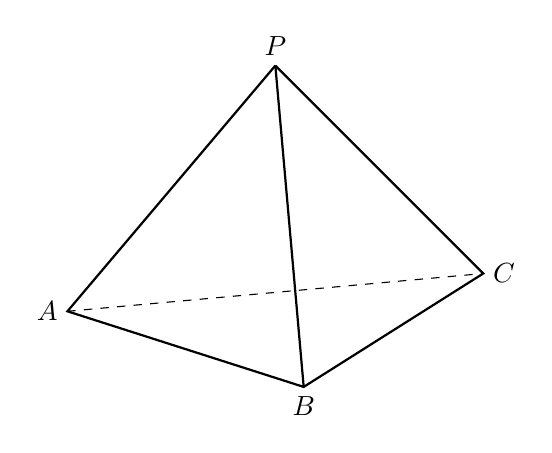
\begin{tikzpicture}[>=stealth,scale=1.2]
  % Coordinates
  \coordinate (A) at (-2.2,-0.4);
  \coordinate (B) at (0.3,-1.2);
  \coordinate (C) at (2.2,0);
  \coordinate (P) at (0,2.2);

  % Edges
  \draw[thick] (P) -- (A) -- (B) -- (C) -- (P);
  \draw[thick] (P) -- (B);
  \draw[dashed] (A) -- (C);

  % Labels
  \node[left] at (A) {$A$};
  \node[below] at (B) {$B$};
  \node[right] at (C) {$C$};
  \node[above] at (P) {$P$};
\end{tikzpicture}
\end{center}
\nopagebreak[4]
（1）求证：$AB\perp BC$；

（2）设 $AB=BC=2\sqrt{3}$，求 $AC$ 与平面 $PBC$ 所成角的大小。

\end{question}
\begin{question}
\gkti{21}（本小题满分 12 分）

设椭圆 $\dfrac{x^2}{m+1}+y^2=1$ 的两个焦点是 $F_1(-c,0)$ 与 $F_2(c,0)$（$c>0$），且椭圆上存在一点 $P$，使得直线 $PF_1$ 与 $PF_2$ 垂直。

（1）求实数 $m$ 的取值范围；

（2）设 $L$ 是相应于焦点 $F_2$ 的准线，直线 $PF_2$ 与 $L$ 相交于点 $Q$，若 $\dfrac{|\overline{QF_2}|}{|\overline{PF_2}|}=2-\sqrt{3}$，求直线 $PF_2$ 的方程。

\end{question}
\begin{question}
\gkti{22}（本小题满分 14 分）

已知数列 $\{a_n\}$ 的前 $n$ 项和 $S_n$ 满足 $S_n=2a_n+(-1)^n$（$n\geqslant 1$）。

（1）写出数列 $\{a_n\}$ 的前三项 $a_1, a_2, a_3$；

（2）求数列 $\{a_n\}$ 的通项公式；

（3）证明：对任意的整数 $m>4$，有 $\dfrac{1}{a_4}+\dfrac{1}{a_5}+\dots+\dfrac{1}{a_m}<\dfrac{7}{8}$。

\end{question}